% chapters/seismo.tex
%
% Copyright 2022 Alexander Lyttle.
%
% This work may be distributed and/or modified under the conditions of the
% LaTeX Project Public License (LPPL) version 1.3 or later.
%
% The latest version of this license is in
% https://www.latex-project.org/lppl.txt and version 1.3 or later is part of
% all distributions of LaTeX version 2005/12/01 or later.
%
%
\chapter{Solar-like oscillators}

\footnote{The spherical harmonic images were computed using code from \url{https://github.com/warrickball/spherical-harmonics}.}

\begin{figure}[tb]
    \centering
    \begin{subfigure}[b]{0.2\linewidth}
        
\includegraphics[width=\linewidth]{figures/spherical_harmonics/0_0.png}
        \caption*{$l=0,\,m=0$}
    \end{subfigure}%
    \begin{subfigure}[b]{0.2\linewidth}
        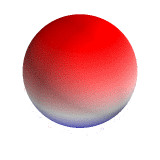
\includegraphics[width=\linewidth]{figures/spherical_harmonics/1_0.png}
        \caption*{$l=1,\,m=0$}
    \end{subfigure}%
    \begin{subfigure}[b]{0.2\linewidth}
        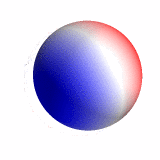
\includegraphics[width=\linewidth]{figures/spherical_harmonics/1_1.png}
        \caption*{$l=1,\,m=1$}
    \end{subfigure}%
    \begin{subfigure}[b]{0.2\linewidth}
        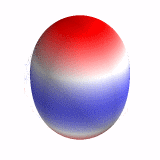
\includegraphics[width=\linewidth]{figures/spherical_harmonics/2_0.png}
        \caption*{$l=2,\,m=0$}
    \end{subfigure}%
    \begin{subfigure}[b]{0.2\linewidth}
        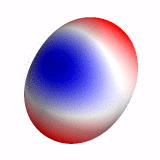
\includegraphics[width=\linewidth]{figures/spherical_harmonics/2_1.png}
        \caption*{$l=2,\,m=1$}
    \end{subfigure}

    \begin{subfigure}[b]{0.2\linewidth}
        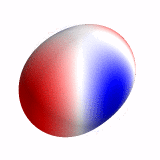
\includegraphics[width=\linewidth]{figures/spherical_harmonics/2_2.png}
        \caption*{$l=2,\,m=2$}
    \end{subfigure}%
    \begin{subfigure}[b]{0.2\linewidth}
        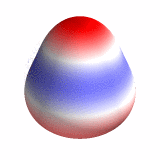
\includegraphics[width=\linewidth]{figures/spherical_harmonics/3_0.png}
        \caption*{$l=3,\,m=0$}
    \end{subfigure}%
    \begin{subfigure}[b]{0.2\linewidth}
        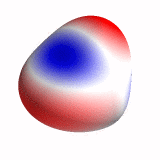
\includegraphics[width=\linewidth]{figures/spherical_harmonics/3_1.png}
        \caption*{$l=3,\,m=1$}
    \end{subfigure}%
    \begin{subfigure}[b]{0.2\linewidth}
        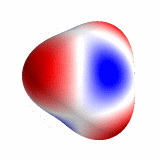
\includegraphics[width=\linewidth]{figures/spherical_harmonics/3_2.png}
        \caption*{$l=3,\,m=2$}
    \end{subfigure}%
    \begin{subfigure}[b]{0.2\linewidth}
        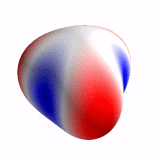
\includegraphics[width=\linewidth]{figures/spherical_harmonics/3_3.png}
        \caption*{$l=3,\,m=3$}
    \end{subfigure}
    \caption{Spherical harmonic modes of oscillation for various combinations of angular degree ($l$) and azimuthal order ($m$).}
    \label{fig:spherical-harmonics}
\end{figure}

\begin{figure}[tb]
    \centering
    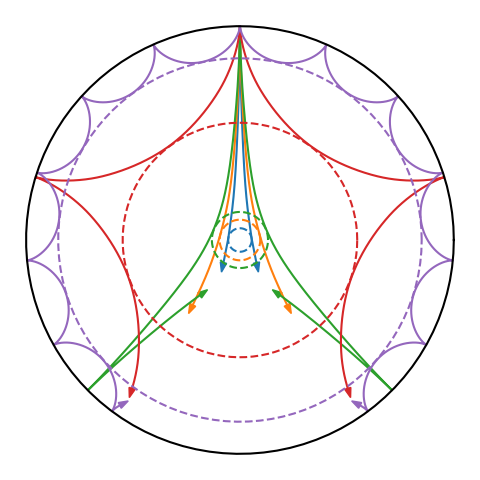
\includegraphics{figures/seismo-wavefronts.png}
    \caption{}
\end{figure}

\begin{figure}[tb]
    \centering
    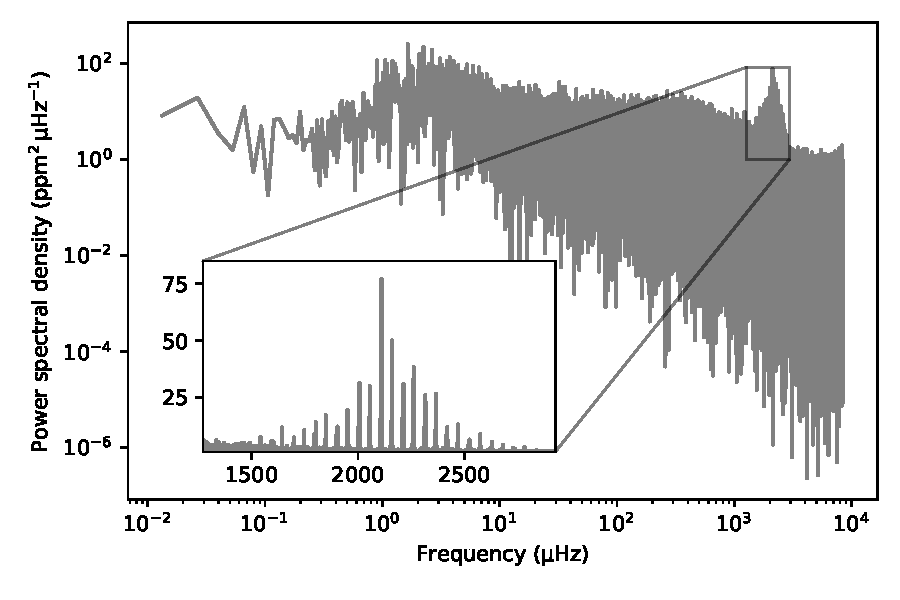
\includegraphics{figures/seismo-psd.pdf}
    \caption{The power spectral density of 16 Cyg A. The inset plot highlights the comb of peaks comprising a Gaussian-like hump in the larger plot.}
\end{figure}

\begin{figure}[tb]
    \centering
    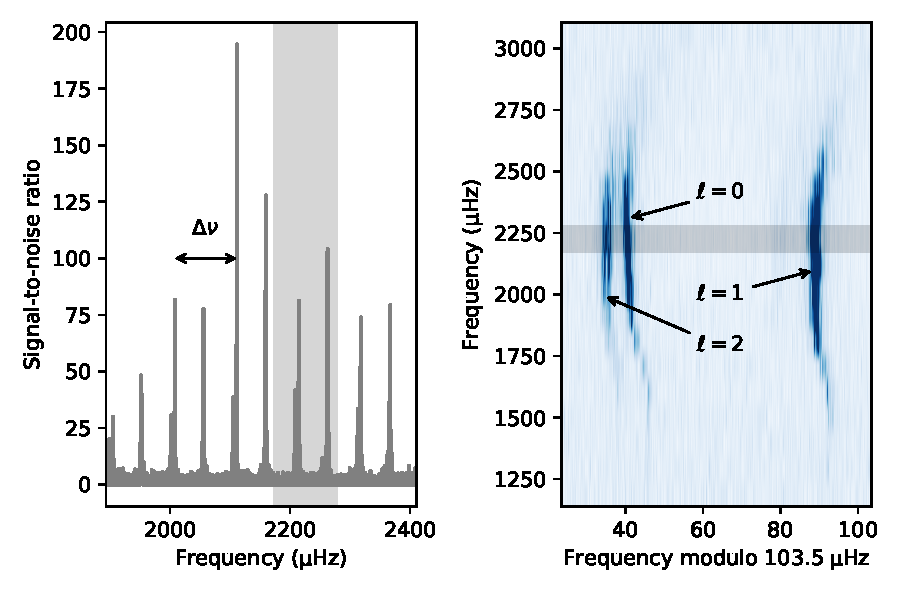
\includegraphics{figures/seismo-echelle.pdf}
    \caption{\emph{Left:} A section of the spectral signal-to-noise ratio (SNR)against frequency for 16 Cyg A. The large frequency spacing (\(\Delta\nu\)) between two radial modes is annotated with a double-headed arrow. The shaded region corresponds to a single row (also highlighted) in the echelle plot (\emph{left}). The echelle plot shows the spectral SNR such that a darker colour represents a higher SNR. Each row spans \SI{103.5}{\micro\hertz} and is stacked in order of frequency. The apparent ridges are labelled according to the angular degree (\(\ell\)) of the modes they represent.}
\end{figure}
